\documentclass{article}
\usepackage[a4paper, margin={3cm, 2.54cm, 2.54cm, 2.54cm}]{geometry}
\usepackage{graphicx}
\usepackage{kotex}
\usepackage{fancyhdr}
\usepackage{mdframed}

\setmainhangulfont{Malgun Gothic}

\pagestyle{fancy}
\fancyhf{}
\lhead{2021 임베디드 소프트웨어 실습 과제}
\rhead{실습 1. 개발환경 익히기}
\lfoot{Typesetted LaTeX from 0x00000FF/CNUCSE-Embedded-Programming-2021-Spring}
\rfoot{페이지 \thepage}

\renewcommand{\headrulewidth}{2pt}
\renewcommand{\footrulewidth}{1pt}

\begin{document}

\paragraph{학번: 201704150}
\paragraph{이름: 허강준}

\section*{문제1 \normalsize\normalfont{프로젝트를 실행하여, Hello.c 파일을 열고 printf문을 수정하여 자신의 학번을 입력한 후 프로젝트를 실행하여 UART\#1 창을 캡처하시오.}}

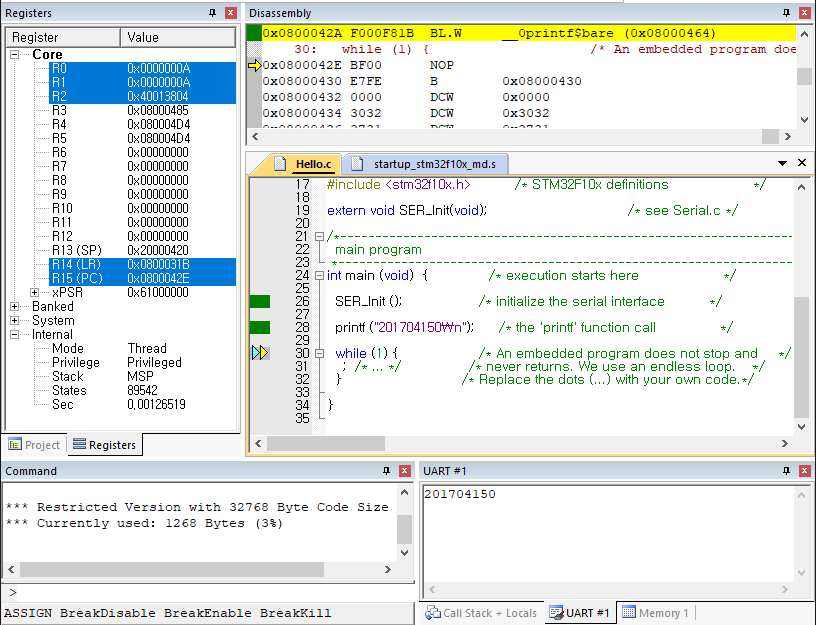
\includegraphics[width=\textwidth]{1.png}

\section*{문제2 \small\normalfont{각 폴더의 역할이 무엇인지, 추측한 내용을 아래에 작성 하시오.}}

\begin{mdframed}
\subsection*{Startup Files}
Target Device의 RESET시 클록 시스템의 재설정, 스택, PC 등의 레지스터 초기화, 인터럽트 벡터 테이블 초기화 및 
프로그램의 진입점으로 분기하는 등 Device 초기화의 전반적인 과정을 수행하는 코드가 보관되는 폴더이다.

\subsection*{System Files}
표준 C 라이브러리 함수를 Target Device에서 사용할 수 있도록 재구현 하거나(Retarget.c), 필요한 라이브러리 
API를 구현하고 노출하는 코드가 보관되는 폴더이다.

\subsection*{Source Files}
사용자 정의 프로그램(user application)을 정의하는 곳으로 Device 초기화 이후 진입점으로 제어가 넘어왔을 때 실행될 코드가 보관된다.

\subsection*{Documentations}
작성한 임베디드 애플리케이션의 스펙이나 API 문서 등을 작성하여 보관하는 폴더이다.
\end{mdframed}

\section*{문제3 \small\normalfont{센서 측정 값을 확인하기 위해서는 Serial Port를 통해 baudrate를 맞춘 후에 
값을 확인해야 한다. Serial.c파일의 \texttt{SER\_Init(void)}함수를 참고하여 baudrate의 값을 쓰시오.}}
\begin{mdframed}
\texttt{Serial.c} 파일의 42번째 라인에 작성된 주석에 따르면 해당 UART 포트는 115200의 baudrate로 작동된다.
\end{mdframed}

\section*{문제4 \small\normalfont{Cortex-M3/M4의 프로세스 모드는 thread 모드와 handler 모드로 구성되어있다. 
thread 모드는 프로세서가 user application을 실행할 때의 동작 모드이고, handler 모드는 프로세서가 OS의 kernel을 
실행하거나 인터럽트를 처리할 때의 동작 모드이다. Register 창을 참조하여 현재 프로세서의 모드가 무엇인지 쓰시오}}
\begin{mdframed}
디버그 모드 실행시 정지하는 \texttt{Reset\_Handler}가 실행되는 시점에서 프로세스 모드는 Thread 모드로 설정된다.
\end{mdframed}

\section*{문제5 \small\normalfont{Cortex-M3/M4는 Privileged과 Unprivileged로 구성된 특권 단계를 갖는다. 
Privileged는 handler 모드와 thread 모드에서 프로세서가 취할 수 있는 상태이며, 모든 시스템 resource와 instruction을 
사용할 수 있다. 또한 handler 모드와 thread 모드 사이의 모드 전환을 수행할 수 있다. Unprivileged는 thread 모드에서만 
프로세서가 취할 수 있는 상태이며 여러 가지 제한을 가진다. 현재의 특권 수준을 쓰시오.}}
\begin{mdframed}
\texttt{Reset\_Handler} 이후 \texttt{main}에 진입한 뒤, 무한 루프 코드까지 진행하였을 때, 특권 수준은 Privileged로 유지되었다.
\end{mdframed}

\section*{문제6 \small\normalfont{Cortex-M3/M4는 MSP(Main Stack Pointer)와 PSP(Process Stack Pointer)라는 
2개의 stack 포인터를 갖는다. MSP는 default stack pointer이지만, 프로세서의 상태가 Privileged일 때만 사용가능하다. 
PSP는 user application에 의해서 사용되기 때문에 thread 모드에서만 사용할 수 있다. 현재의 스택의 종류를 쓰시오.}}
\begin{mdframed}
디버그 실행시 프로세서는 Privileged 모드에서 \texttt{MSP}를 사용하고 있다.
\end{mdframed}

\section*{문제7 \small\normalfont{R15(PC)는 Program Counter로 다음에 수행이 되어야 할 명령어의 주소를 가리킨다.
 Debug 상태에서  
\includegraphics{2.png}(Reset)버튼을 누른 후 PC값이 얼마인지 쓰시오.}}
 \begin{mdframed}
RESET시 PC는 \texttt{0x08000100}로 설정되었다.
 \end{mdframed}

\section*{문제8 \small\normalfont{View 메뉴의 Memory 윈도우 Memory 1을 열고, On-Chip IROM1 영역의 시작 주소를 
0x 형태로 입력하면, 메모리 내용을 볼 수 있다. 0x8000100주소를 입력하여 데이터를 2바이트씩 4개의 데이터를 쓰시오. 
Little Endian이라는 점에 주의하시오.}}
\begin{mdframed}
\begin{itemize}
    \item 주소:0x8000100 \hspace{3cm} 데이터:\texttt{0x4806}
    \item 주소:0x8000102 \hspace{3cm} 데이터:\texttt{0x4780}
    \item 주소:0x8000104 \hspace{3cm} 데이터:\texttt{0x4806}
    \item 주소:0x8000106 \hspace{3cm} 데이터:\texttt{0x4700}
\end{itemize}
\end{mdframed}

\section*{문제9 \small\normalfont{Hello 프로젝트를 실행하면, \texttt{startup\_stm32f10x\_md.s} 파일에서 프로그램이
 시작해서 Hello.c 의 main 까지 프로그램이 진행된다. 프로그램의 시작부터 Hello 메시지를 출력하기 까지 프로그램의 
 실행과정을 조사해서 진행과정을 설명하시오. }}
 \begin{mdframed}
    \begin{itemize}
        \item 스택, 힙 크기 설정 및 할당
        \item 내/외부 인터럽트 벡터 테이블 초기화
        \item \texttt{Reset\_Handler} 호출
            \begin{itemize}
                \item \texttt{SystemInit}을 호출하여 클록 시스템, 레지스터 등 초기화
                \item \texttt{\_\_main} 라이브러리 함수로 분기
                \item \texttt{main()} 호출함으로서 user application으로 control 이동
            \end{itemize}
    \end{itemize}
 \end{mdframed}
\end{document}